\documentclass[border=3pt,tikz]{standalone}
\usepackage[utf8]{vietnam}
\usetikzlibrary{calc,angles,intersections,shapes.geometric,arrows,decorations.markings,arrows.meta,patterns.meta,patterns}
\usepackage{tikz-3dplot,pgfplots}
\pgfplotsset{compat=1.15}
\usepgfplotslibrary{polar}
\usepackage{amsmath}
\begin{document}
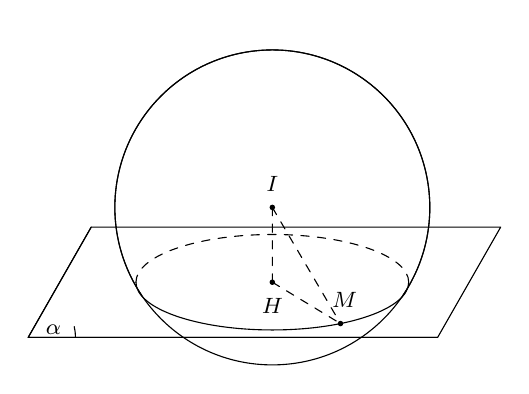
\begin{tikzpicture}[scale=1,>=stealth, font=\footnotesize, line join=round, line cap=round]
	\def \x{2} %bán kính trục lớn elip
	\def \y{0.7} %bán kính trục bé elip
	\path
	(0:0) coordinate (I)
	(\x,0) coordinate (B)
	(-\x,0) coordinate (A)
	($(0,-0.5*\x)+(0,0.05)$) coordinate (H)
	($(H)+(-60:\x*0.866 cm and \y*0.866 cm)$) coordinate (M)
	($(H)+(-\x-1.1,-\y)$) coordinate (m)
	($(H)+(\x+0.1,-\y)$) coordinate (n)
	($(H)+(\x+0.9,\y)$) coordinate (p)
	($(m)+(p)-(n)$) coordinate (q)
	;
	\path [name path=pq] (p) -- (q);
	\path [name path=mn] (m) -- (n);
	\draw[name path=circ1] (0,0) circle (2);
	\path[name intersections={of=circ1 and pq}](intersection-1) coordinate (p') (intersection-2)coordinate (q');
	\path[name intersections={of=circ1 and mn}](intersection-1) coordinate (x) (intersection-2) coordinate (y);
	\draw (-34:\x) arc (-34:214:\x);
	\draw[dashed] ($(-30:\x)+(0,0.05)$) arc (0:180:\x*0.866 cm and \y*0.866 cm);
	\draw ($(-30:\x)+(0,0.05)$) arc (0:-180:\x*0.866 cm and \y*0.866 cm);
	\draw[dashed] (I)--(H) (I)--(M) (H)--(M);
	\draw (q')--(q)--(m)--(n)--(p)--(p');
	\foreach \p/\q in {I/90,H/-90,M/80}{
		\path (\p) node[shift={(\q:3mm)}]{$\p$ };
		\fill[black] (\p) circle (1.0pt);
	}
	\draw (n)--(m)--(q) pic[draw,angle radius=6mm]{angle=n--m--p}; \node at ($(m)+(0.1,0.1)$)[right]{$\alpha$};
\end{tikzpicture}

\begin{tikzpicture}[join=round, cap=round]
	\def\R{4}
	\def\go{-30}
	\def\gi{-15}
	\pgfmathsetmacro\a{\R*sin(60+\gi)}
	\pgfmathsetmacro\b{.15*\a}
	\path
	(0,0)coordinate(I)
	({\gi-30}:\R)coordinate(A)
	({180-\gi+30}:\R)coordinate(B)
	(A)--(B)coordinate[pos=.5](H)
	(A)arc(0:\go:{\a} and {\b})coordinate(M)
	(0:.6*\R)+(\gi:\R)coordinate(P)
	(180:.4*\R)+({-180-\gi}:\R)coordinate(Q)
	({\gi}:\R)coordinate(C)
	({180-\gi}:\R)coordinate(D)
	(Q)--(H)coordinate[pos=2](P')
	(P)--(H)coordinate[pos=2](Q');
	\draw[densely dashed](H)--(I)(I)--(M)--(H)(C)--(D);
	\draw[densely dotted](A)arc(0:180: {\a} and {\b})
	(A)arc({\gi-30}:{-180+\gi-30}:{\R});
	\draw(A)arc({\gi-30}:{180-\gi+30}:\R)
	(A)arc(0:-180: {\a} and {\b})
	(P')--(Q')(D)--(Q)--(Q')(C)--(P)--(P');
	\draw[brown](Q')+(0:.4)arc(0:{-2*\go-\gi}:.4);
	\path(Q')+(35:.2)node[scale=.8]{$\alpha$};
	\foreach \d/\g in{H/180,M/-90,I/180}\draw[fill=white](\d)circle(1pt)+(\g:0.35)node{$\d$};
\end{tikzpicture}
\end{document}